\subsection{Syntax units}
\label{sec:syntax-units}

\begin{figure*}[ht]
    \centering
    \begin{subfigure}{0.49\textwidth}
            \centering
            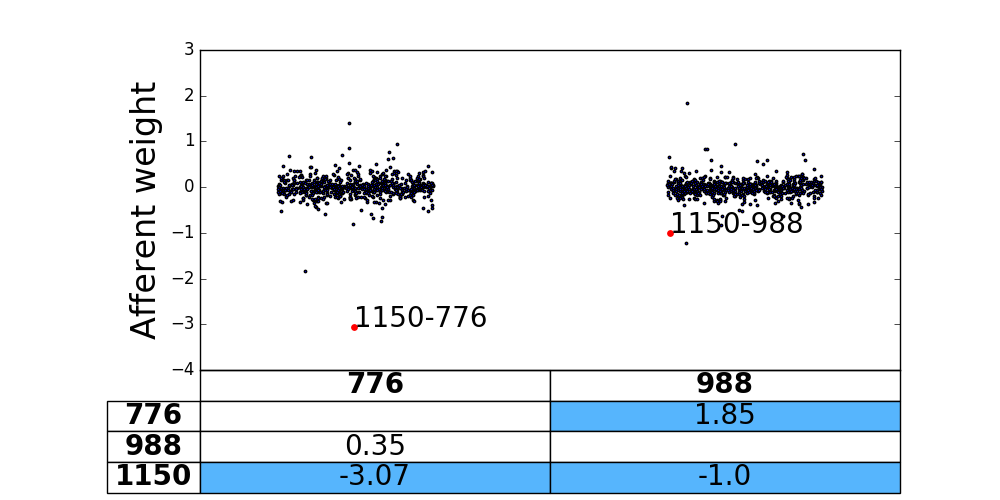
\includegraphics[height=3.3cm,width=\textwidth]{Figures/gate_Input_afferent_interactions.png}
            \caption{Input gate}
            \label{fig:interaction-input}
    \end{subfigure}
    \begin{subfigure}{0.49\textwidth}
           \centering
          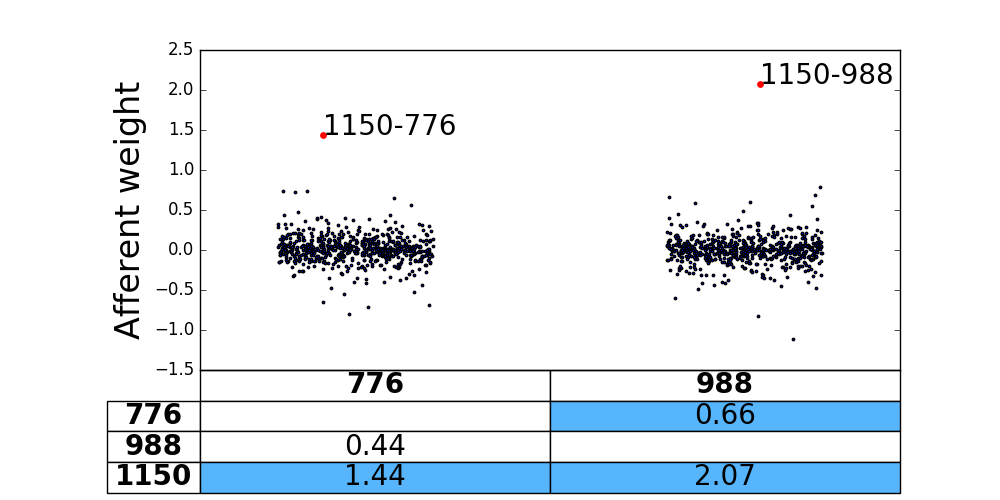
\includegraphics[height=3.3cm,width=\textwidth]{Figures/gate_Forget_afferent_interactions.png}
          \caption{Forget gate}
          \label{fig:interaction-forget}
    \end{subfigure}
    \caption{Connectivity among the syntax unit \unit{2}{500} and
      LR-number units \unit{2}{126} and \unit{2}{338}. Projecting
      units are on the table rows. Blue background highlights outlier
      values ($|z-score|>3$). Weights from the syntax unit are marked in red
      and are explicitly labeled in the plots, which show the overall distributions of afferent weights to each number unit.}
\label{fig:interaction}
\end{figure*}

We saw how the input and forget gates of the LR-number units control the flow of subject-number information. It remains unclear, however, how the dynamics of these gates are controlled by the network. We hypothesized that other units in the network may encode information about the syntactic structure of the sentence, and thus about the subject-verb dependency. These units could then control and coordinate the opening and closing of the input and forget gates of the number units. 

To identify such 'syntax' units, we tested from which units syntactic information can be efficiently decoded. We used depth of the syntactic tree as a proxy for syntactic structure \cite{Nelson:etal:2017} and trained an L2-regularized regression model to predict syntactic tree-depth from the hidden-state activity of all units. In all experiments, we used the data presented in Section \ref{sec:the_data} above and performed a nested 5-fold cross-validation procedure. Word frequency, which was added as a covariate to the model, had a negligible effect on the results. Syntactic tree-depth was found to be efficiently decodable from network activity ($R^2_{test-set}=0.85\pm0.009$; covariate-corrected). A small subset of `syntax' units had relatively high weights in the regression model (mean weight = $7.6\times{}10^{-4}$, SD=$7.86\times{}10^{-2}$; cutoff for outlier weights was set to three SDs). Since the interpretation of the regression weights may depend on possible correlations among the features, we also tested the causal effect of these units on NA-task performance. Ablating the syntax units together resulted in significant performance reduction in NA-tasks that have an interfering noun: Linzen NA-task: $p=0.024$, nounPPAdv-SP: $p=0.011$, nounPPAdv-PS: $p=0.034$, nounPP-SP: $p<0.001$ and marginally significant in nounPP-PS: $p=0.052$ (compared to 1000 random ablations of subsets of units of the same size).

To gain further insight regarding the functioning of the syntax units, we next visualized their gate and cell dynamics during sentence processing. We found that cell activity of unit \unit{2}{500}, which also had one of the highest weights in the regression model, was remarkably structured. The activity of
this unit increases across the entire subject-verb dependency and drops abruptly right after. Figures
\ref{fig:syntax-unit-2Adv} and \ref{fig:syntax-unit-nounpp} show cell activity of this unit during the processing of stimuli from the 2Adv and nounPP tasks. We found the same dynamics in cases where another
verb occurs between subject and main verb, as in subject relatives (Figure \ref{fig:syntax-unit-subjrel}), and in exceptionally long-distance dependencies with two interfering nouns and verbs (Figure \ref{fig:syntax-unit-double-subjrel}). Taken together, these results suggest that unit \unit{2}{500} consistently encodes subject-verb dependencies in a syntax-sensitive manner. Other syntax units did not show an easily interpretable dynamics and had no clear interactions with the number units in the analysis discussed next. This suggests that they perform different syntactic, or possibly other, functions.
